%%%%%%%%%%%%%%%%%%%%%%%%%%%%%%%%%%%%%
%                                   %
% Compile with XeLaTeX and biber    %
%                                   %
% Questions or comments:            %
%                                   %
% joshua dot mcneill at uga dot edu %
%                                   %
%%%%%%%%%%%%%%%%%%%%%%%%%%%%%%%%%%%%%

\documentclass{beamer}
  % Read in standard preamble (cosmetic stuff)
  %%%%%%%%%%%%%%%%%%%%%%%%%%%%%%%%%%%%%%%%%%%%%%%%%%%%%%%%%%%%%%%%
% This is a standard preamble used in for all slide documents. %
% It basically contains cosmetic settings.                     %
%                                                              %
% Joshua McNeill                                               %
% joshua dot mcneill at uga dot edu                            %
%%%%%%%%%%%%%%%%%%%%%%%%%%%%%%%%%%%%%%%%%%%%%%%%%%%%%%%%%%%%%%%%

% Beamer settings
% \usetheme{Berkeley}
\usetheme{CambridgeUS}
% \usecolortheme{dove}
% \usecolortheme{rose}
\usecolortheme{seagull}
\usefonttheme{professionalfonts}
\usefonttheme{serif}
\setbeamertemplate{bibliography item}{}

% Packages and settings
\usepackage{fontspec}
  \setmainfont{Charis SIL}
\usepackage{hyperref}
  \hypersetup{colorlinks=true,
              allcolors=blue}
\usepackage{graphicx}
  \graphicspath{{../../figures/}}
\usepackage[normalem]{ulem}
\usepackage{enumerate}

% Document information
\author{M. McNeill}
\title[FREN2001]{Français 2001}
\institute{\url{joshua.mcneill@uga.edu}}
\date{}

%% Custom commands
% Lexical items
\newcommand{\lexi}[1]{\textit{#1}}
% Gloss
\newcommand{\gloss}[1]{`#1'}
\newcommand{\tinygloss}[1]{{\tiny`#1'}}
% Orthographic representations
\newcommand{\orth}[1]{$\langle$#1$\rangle$}
% Utterances (pragmatics)
\newcommand{\uttr}[1]{`#1'}
% Sentences (pragmatics)
\newcommand{\sent}[1]{\textit{#1}}
% Base dir for definitions
\newcommand{\defs}{../definitions}


  % Packages and settings

  % Document information
  \subtitle[Heures et verbes \lexi{-ir}]{Les heures et les verbes \lexi{-ir}}

\begin{document}
  % Read in the standard intro slides (title page and table of contents)
  \begin{frame}
    \titlepage
    \tiny{Office: % Basically a variable for office hours location
Gilbert 121\\
          Office hours: % Basically a variable for office hours
 lundi, mercredi, vendredi 10:10--11:10
}
  \end{frame}

  \begin{frame}{Annonces}
    \begin{itemize}
      \item Pas de cours le 28 octobre (vendredi)!
      \item[] \tinygloss{No classes October 28th (Friday)!}
    \end{itemize}
  \end{frame}

  \begin{frame}[t]{Des comparaisons}
    \only<1-2>{
      Qui est plus grand? \underline{\uncover<2>{Lebron James (6'9'')}}
    }
    \only<3-4>{
      Qui est plus chic? \underline{\uncover<4>{Cyndi Lauper}}
    }
    \only<5-6>{
      Quel ordinateur est moins cher? \underline{\uncover<6>{le PC}}
    }
    \only<7-8>{
      Quel cours est moins facile? \underline{\uncover<8>{les mathématiques}}
    }
    \only<9-10>{
      Quel bâtiment est plus vieux? \underline{\uncover<10>{la cathédrale Notre-Dame de Paris (1345)}}
    }
    \only<11-12>{
      Qui est plus fort? \underline{\uncover<12>{George Foreman}}
    }
    \vspace{0.5cm}
    \begin{columns}
      \column{0.5\textwidth}
        \begin{center}
          \only<1-2>{
            
\includegraphics[scale=0.13]{lebron.jpg}
          }
          \only<3-4>{
            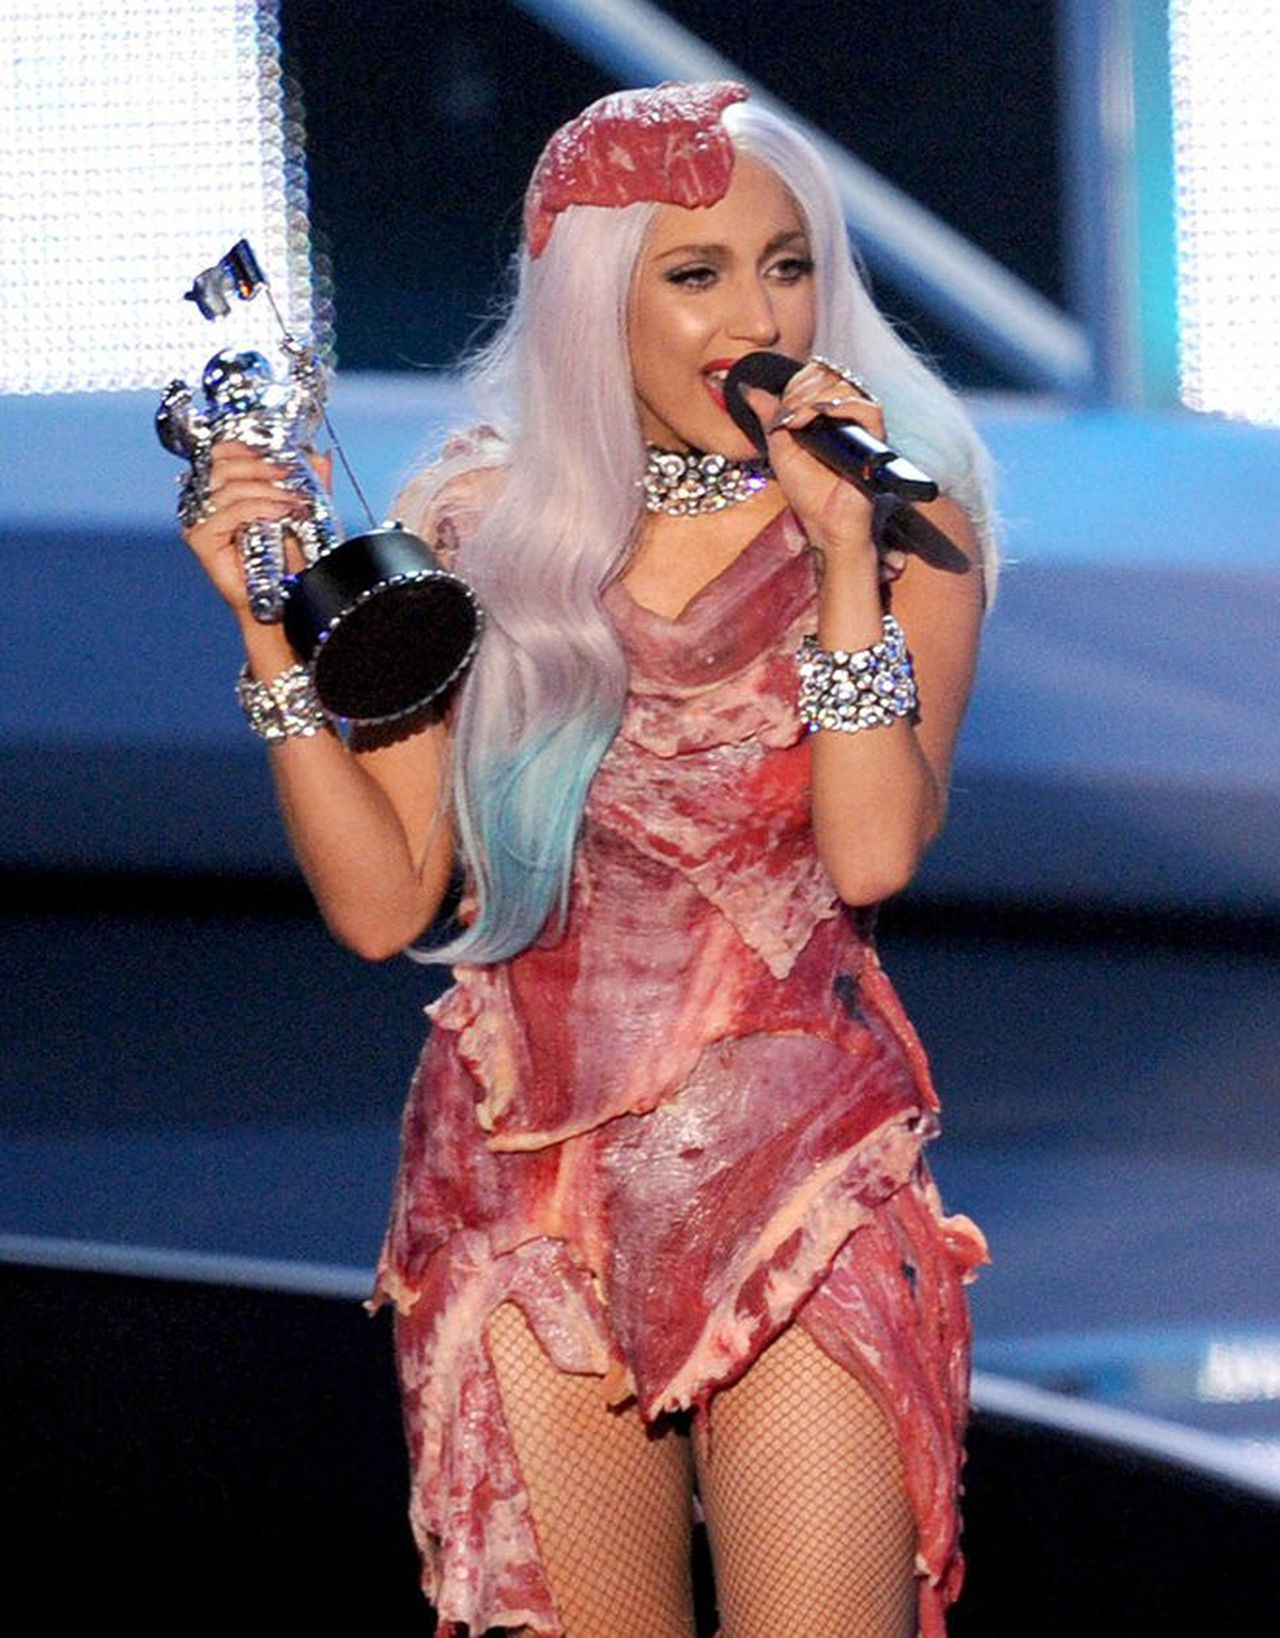
\includegraphics[scale=0.09]{lady_gaga.jpg}
          }
          \only<5-6>{
            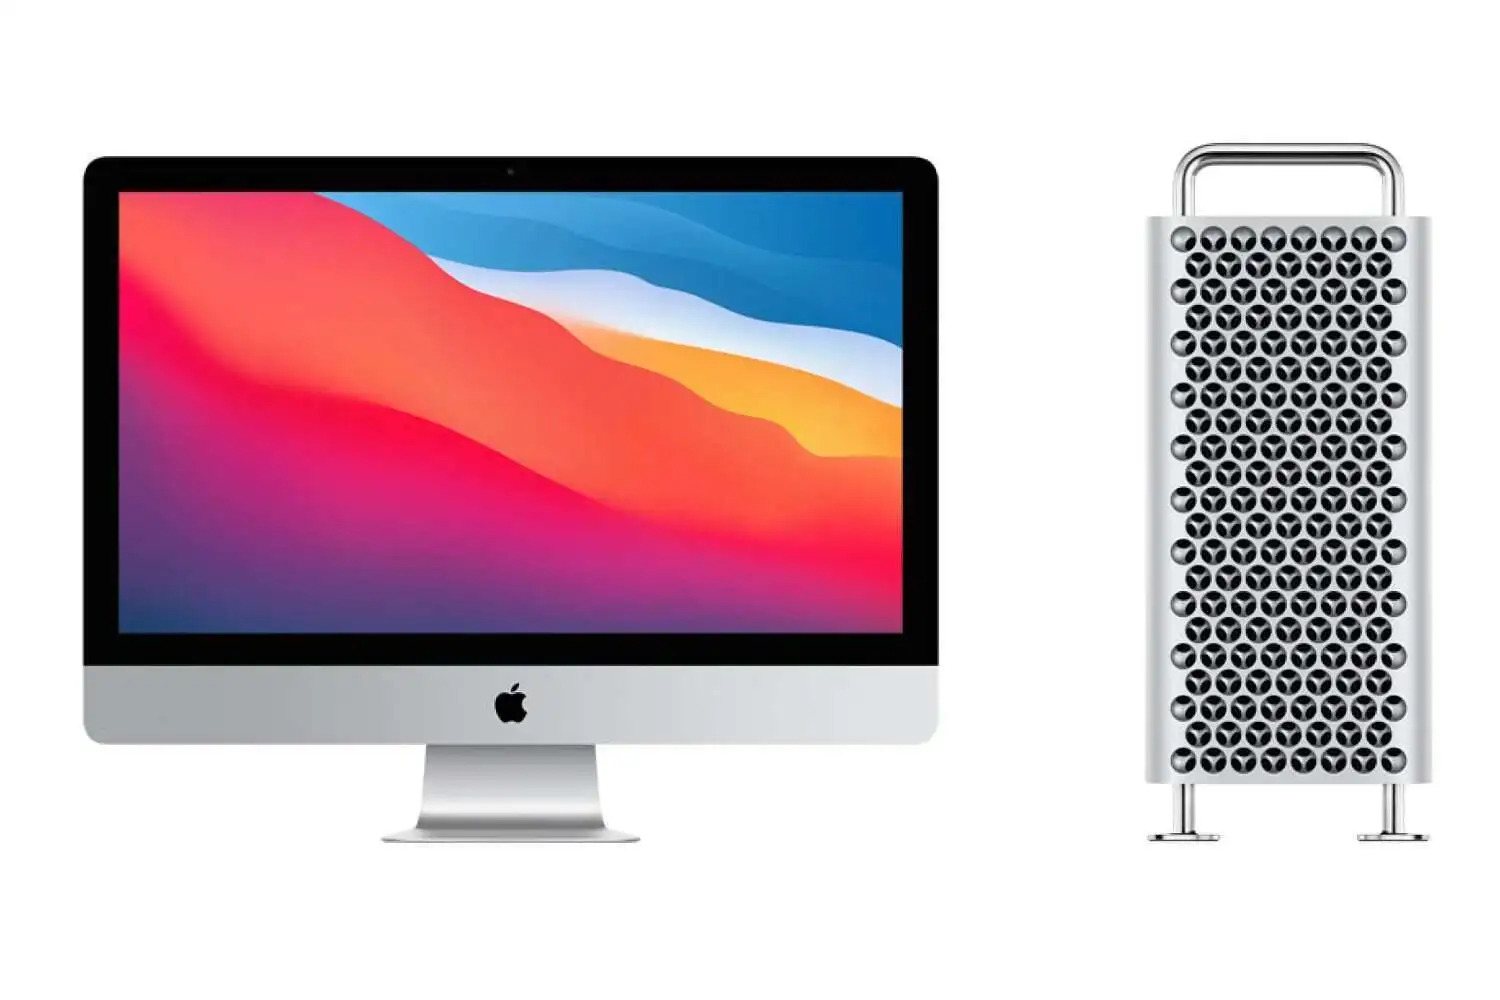
\includegraphics[scale=0.12]{mac.jpg}
          }
          \only<7-8>{
            \includegraphics[scale=0.2]{français.jpg}
          }
          \only<9-10>{
            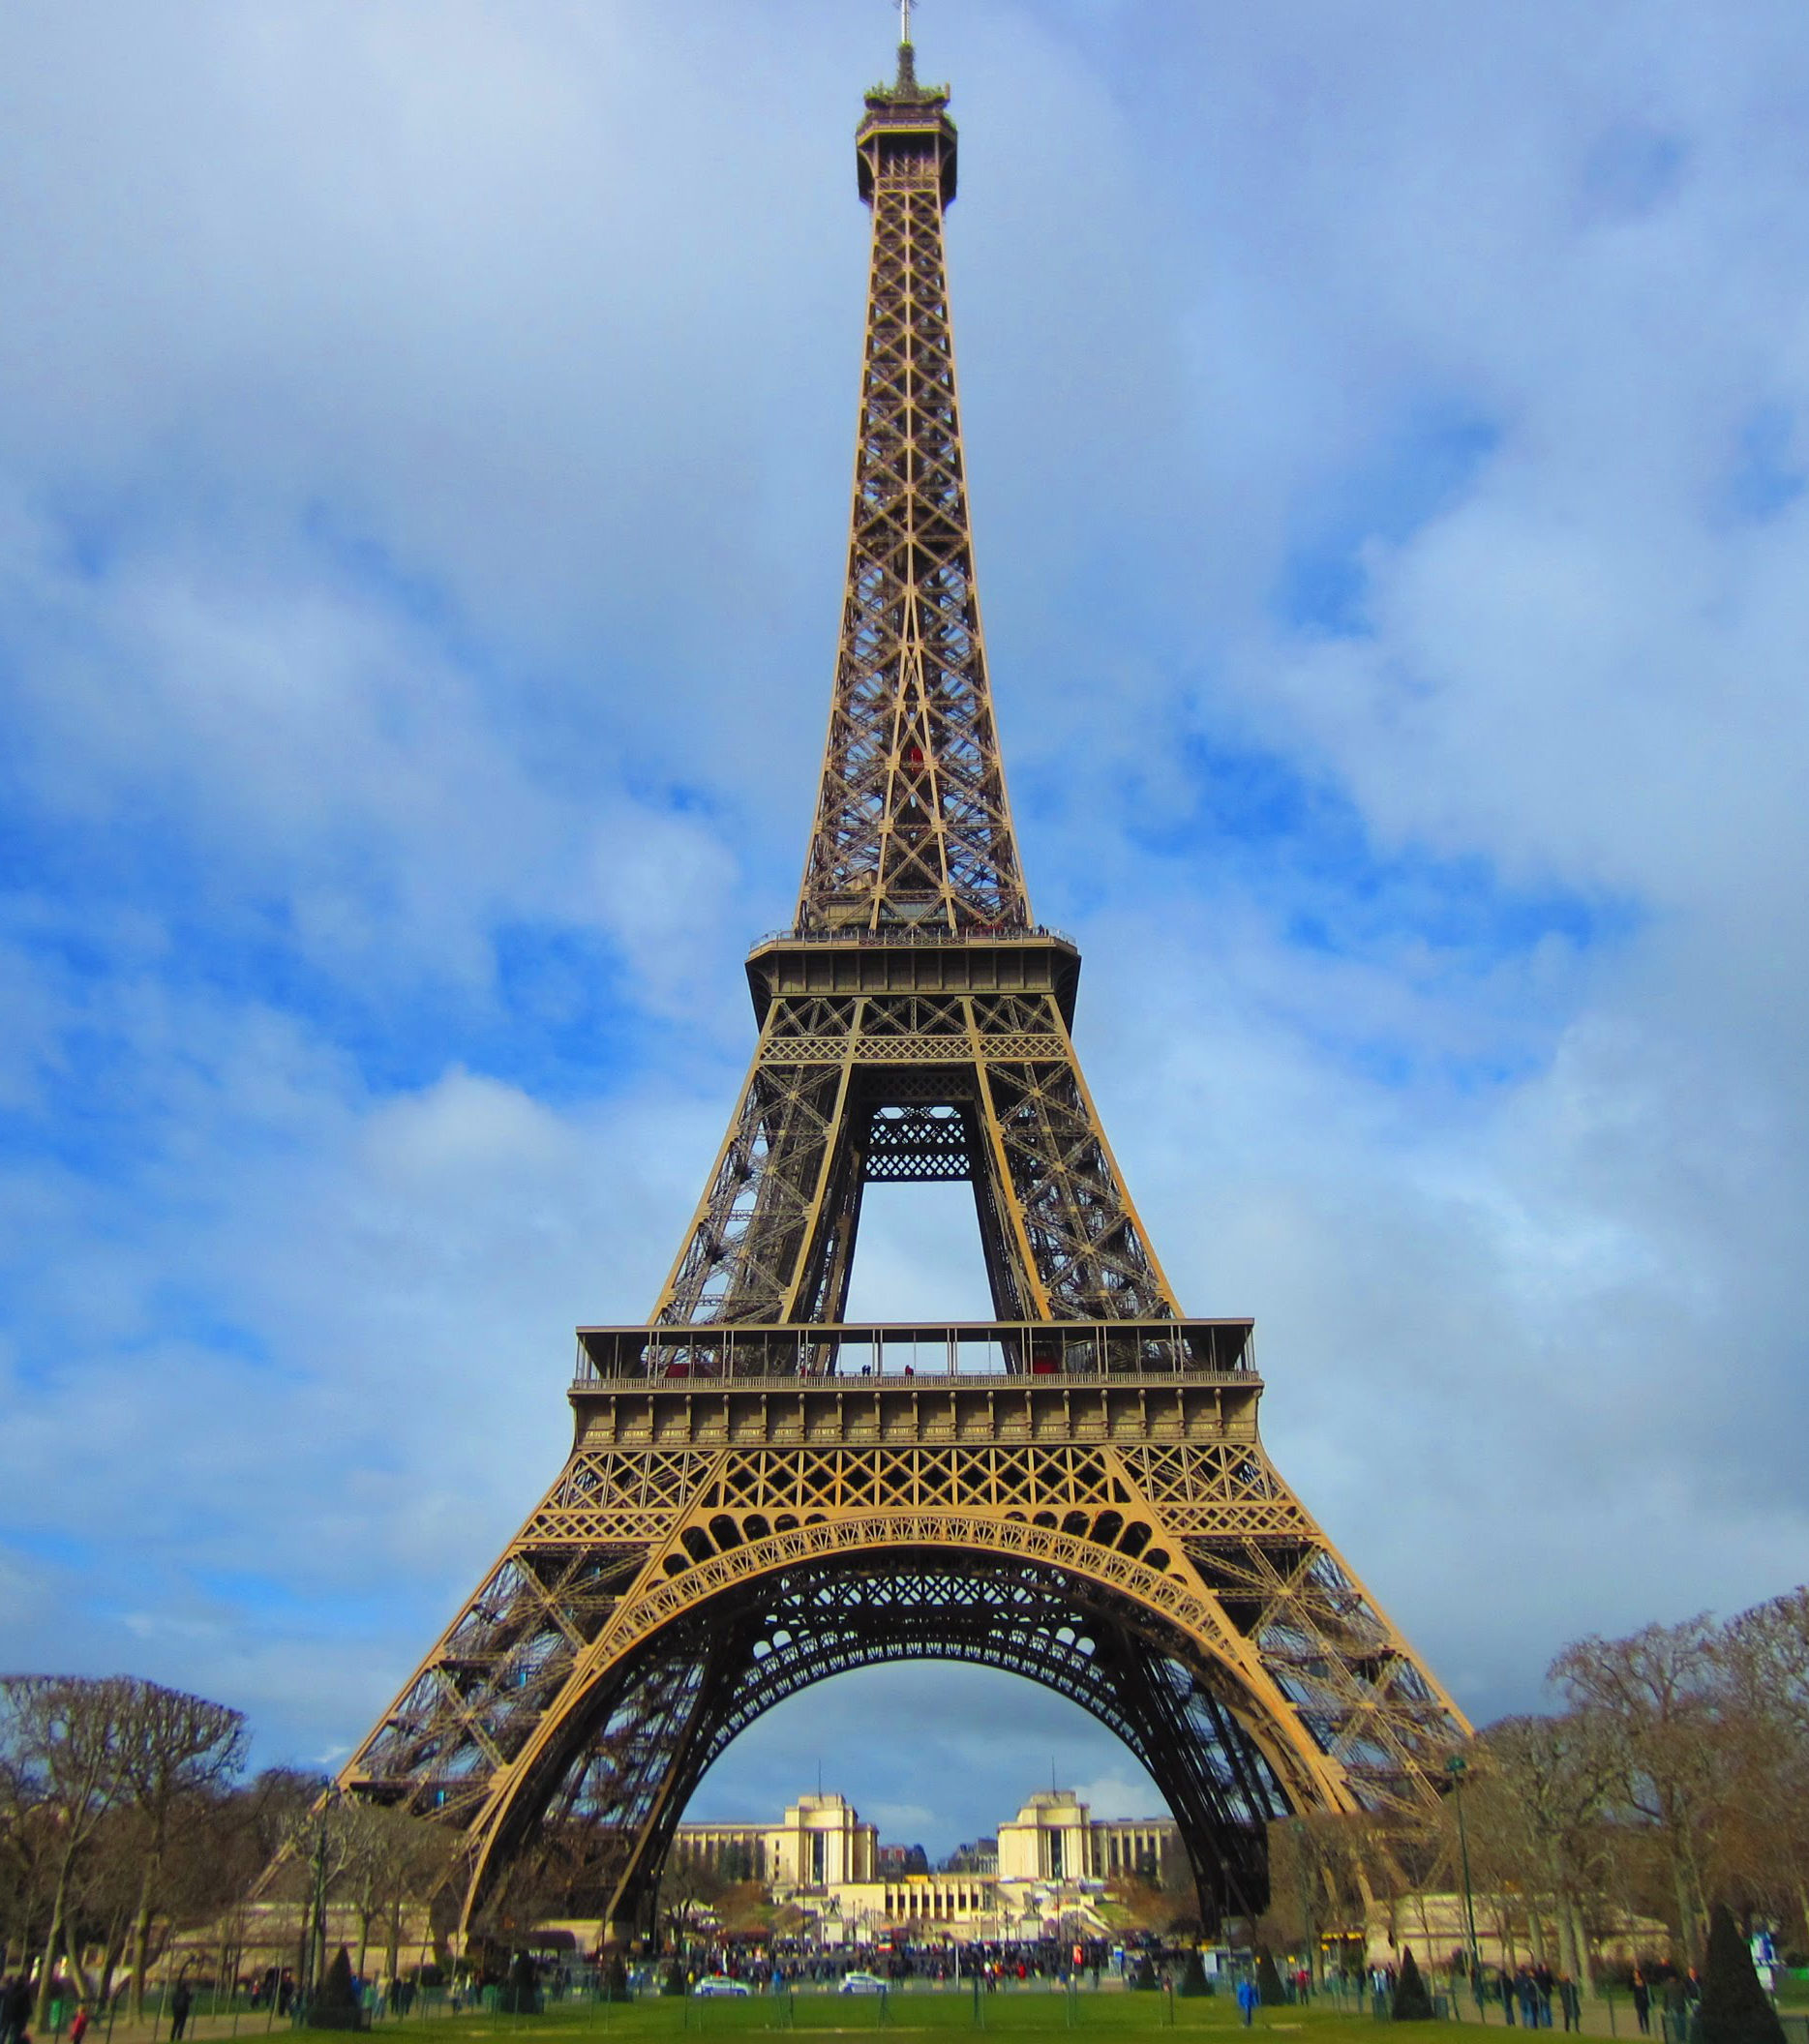
\includegraphics[scale=0.067]{tour_eiffel.jpg}
          }
          \only<11-12>{
            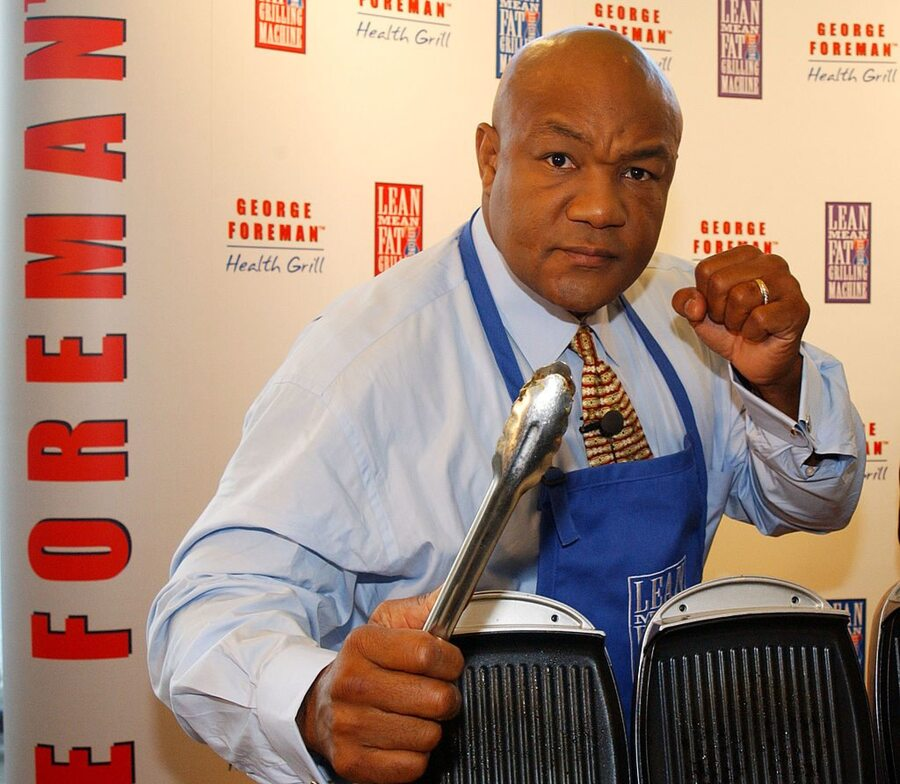
\includegraphics[scale=0.15]{foreman.jpg}
          }
        \end{center}
      \column{0.5\textwidth}
        \begin{center}
          \only<1-2>{
            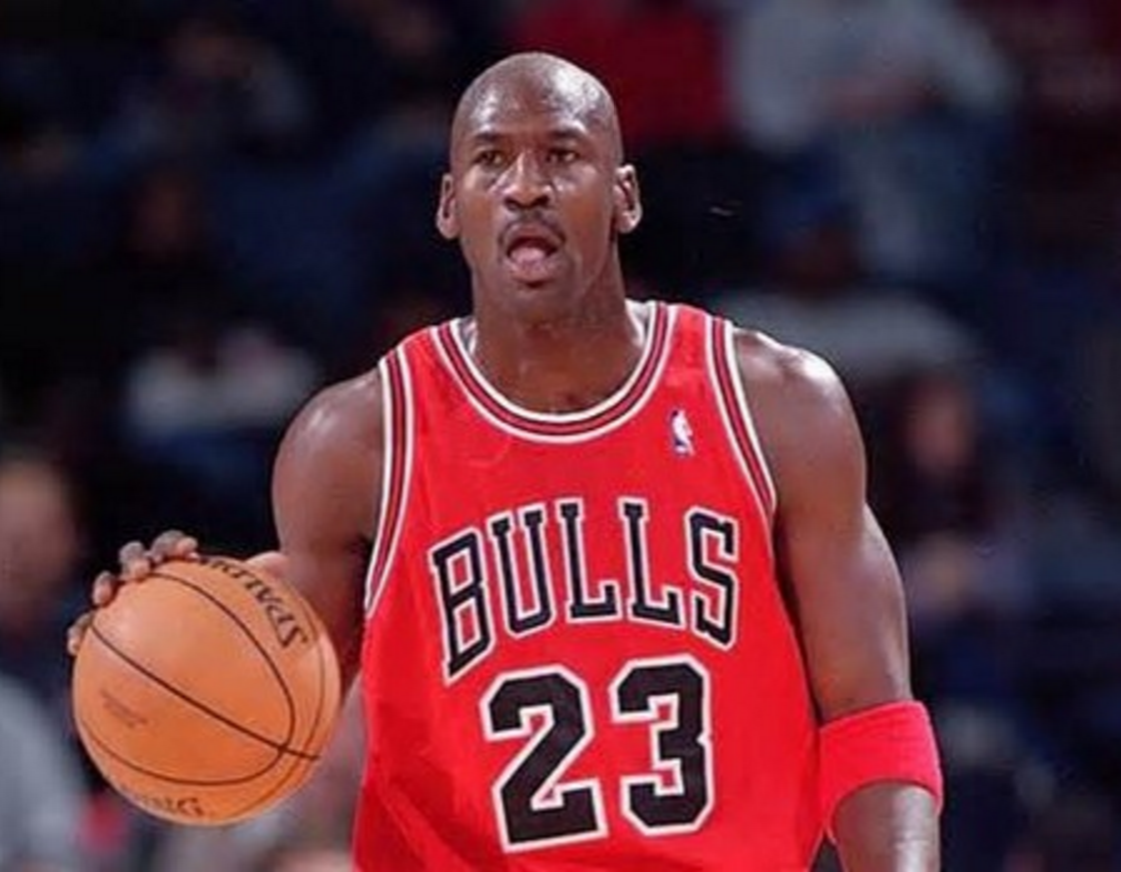
\includegraphics[scale=0.14]{jordan.png}
          }
          \only<3-4>{
            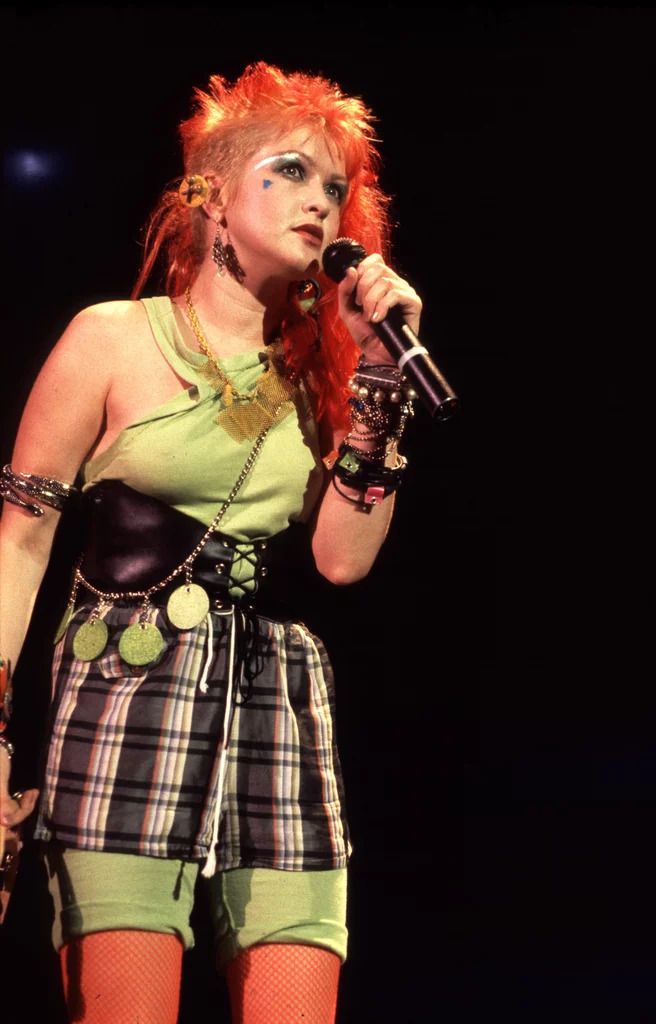
\includegraphics[scale=0.15]{cyndi_lauper.jpg}
          }
          \only<5-6>{
            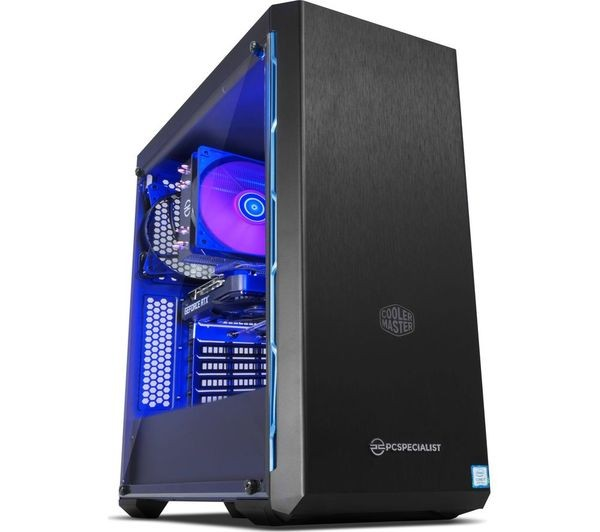
\includegraphics[scale=0.27]{pc.jpg}
          }
          \only<7-8>{
            
\includegraphics[scale=0.125]{maths.jpg}
          }
          \only<9-10>{
            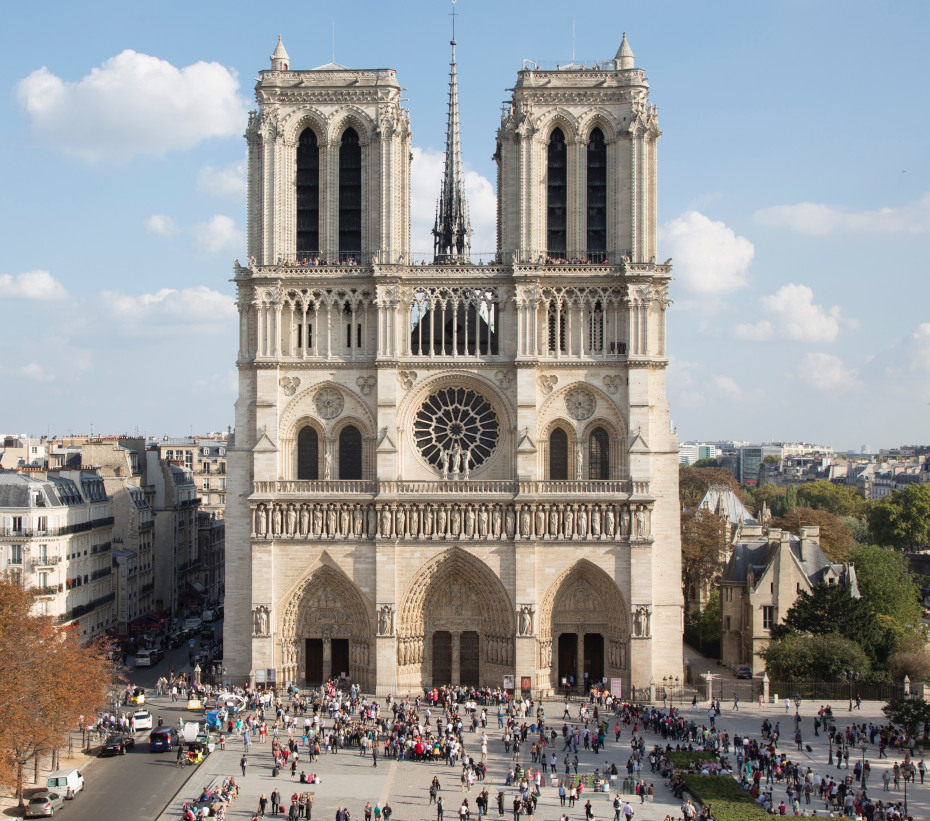
\includegraphics[scale=0.75]{notre_dame.jpg}
          }
          \only<11-12>{
            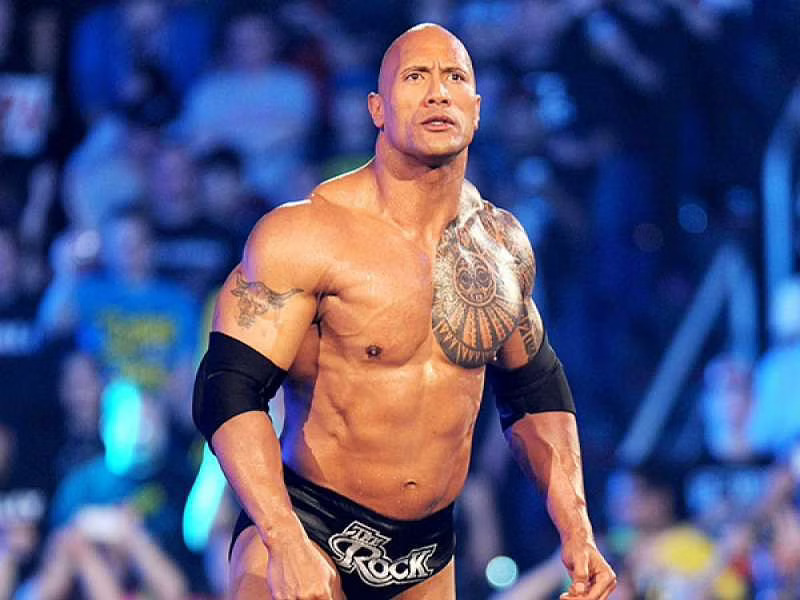
\includegraphics[scale=0.2]{therock.jpg}
          }
        \end{center}
    \end{columns}
  \end{frame}

  \begin{frame}{}
    \begin{center}
      \Large Quiz
    \end{center}
  \end{frame}

  \begin{frame}{Le mieux}
    Avec un/e partenaire, répondez aux questions, et comparez vos réponses. \\
    \tinygloss{With a partner, answer the questions, and compare your answers.}
    \begin{columns}
      \scriptsize
      \column{0.45\textwidth}
        \begin{description}
          \item[] \textbf{Modèle:}
          \item[] \lexi{Qui nage mieux, toi ou ton père/ta mère?}
          \item[E1:] Je nage moins bien que mon père.
          \item[E2:] Pas moi. Je nage mieux que mon père. Il n'aime pas nager!
        \end{description}
      \column{0.55\textwidth}
        \begin{enumerate}
          \item Qui chante mieux, toi ou ta sœur/ton frère?
          \item Qui fait mieux la cuisine, ta mère ou ton père?
          \item Qui danse mieux, toi et tes amis ou tes parents et leurs amis?
          \item Qui joue mieux au basket, toi ou ta sœur/ton frère?
          \item Qui s'habille mieux, toi ou ton meilleur ami/ta meilleure amie?
          \item Qui travaille mieux, toi ou tes colocataires?
          \item Qui joue mieux au golf, toi ou tes parents?
        \end{enumerate}
    \end{columns}
  \end{frame}

  \begin{frame}{Vrai ou faux?}
    Avec un/e partenaire, explique la raison que la phrase est vraie ou fausse pour toi. \\
    \tinygloss{With a partner, explain the reason why the phrase is true or false for you.}
    {\scriptsize
    \begin{description}
      \item[] \textbf{Modèle:} \lexi{Numéro 1}
      \item[E1:] C'est vrai. Je me lève à 7 heures, et mon colocataire se lève à 8 heures.
      \item[E2:] C'est faux. Mon colocataire se lève plus tôt que moi pour aller aux cours.
    \end{description}
    \begin{enumerate}
      \item Je me lève plus tôt que mon/ma colocataire.
      \item Mon/Ma colocataire travaille mieux que moi.
      \item Je travaille plus tard la nuit que mon/ma colocataire.
      \item Je sors plus souvent que mon/ma colocataire.
      \item Je vais moins souvent à la bibliothèque que mon/ma colocataire.
      \item Mon/Ma colocataire part plus souvent que moi le week-end.
      \item Mon/Ma colocataire dort moins profondément que moi.
      \item Je regarde moins souvent ma montre que mon/ma colocataire.
    \end{enumerate}
    }
  \end{frame}

  \begin{frame}{}
    \begin{center}
      \Large Questions?
    \end{center}
  \end{frame}
\end{document}
